% !TEX root = Master.tex

The procedure is continued also for key category cluster 8 with the same conditions, since we have similar issues as in the previous two clusters.
\\

\autoref{tab:estimated_parameters_kcc_8_no_covariates}, \autoref{fig:kcc_8_marginal} and \autoref{fig:res_kcc_8_no_covariates} summarize the findings when the log-sales of \ac{KCC} 8 are fitted to an ex-Gaussian distribution with no regressors. Normality of the residuals can be assumed, as the Shapiro-Wilk test returns a p-value of 0.99 and thus fails to reject the null hypothesis of non-normality.
\\



\begin{table}[H]
\setlength\arrayrulewidth{1pt}  
\centering
\begin{adjustbox}{max width=\textwidth}\
\begin{tabular}{|c|c|c|}
\hline
\rowcolor{lightgray} 
$\hat{\mu}$ & $\hat{\sigma}$ & $\hat{\nu}$ \\ \hline
7.21        & 0.27           & 0.46        \\ \hline
\end{tabular}
\end{adjustbox}
\caption{Estimated parameters for log-sales of KCC 8 fitted to ex-Gaussian distribution with no covariate effects}
\label{tab:estimated_parameters_kcc_8_no_covariates}
\end{table}



 \begin{figure}[H]
\centering
\begin{subfigure}{.45\textwidth}
  \centering
  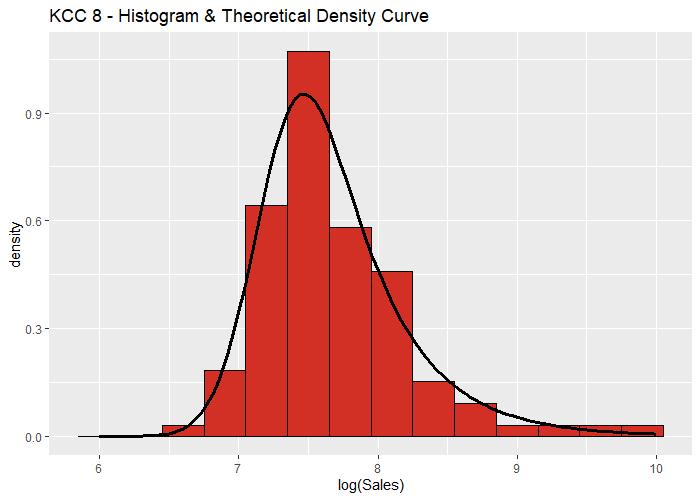
\includegraphics[width=\linewidth]{figures/kcc_8_density.png}
  \caption{Histogram \& theoretical density}
  \label{fig:kcc_8_density}
\end{subfigure}
\begin{subfigure}{.45\textwidth}
  \centering
  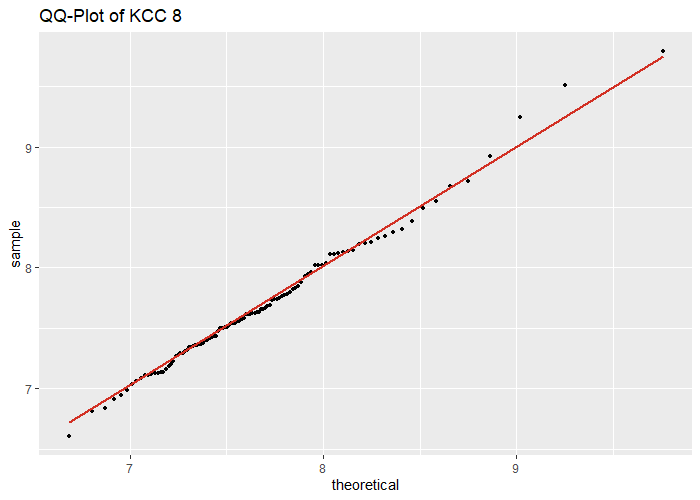
\includegraphics[width=\linewidth]{figures/kcc_8_qqplot.png}
  \caption{QQ-Plot}
  \label{fig:kcc_8_qqplot}
\end{subfigure}
\caption{ex-Gaussian distribution fitted to log-sales of \ac{KCC} 8}
\label{fig:kcc_8_marginal}
\end{figure} 


\begin{figure}[H]
\centering
  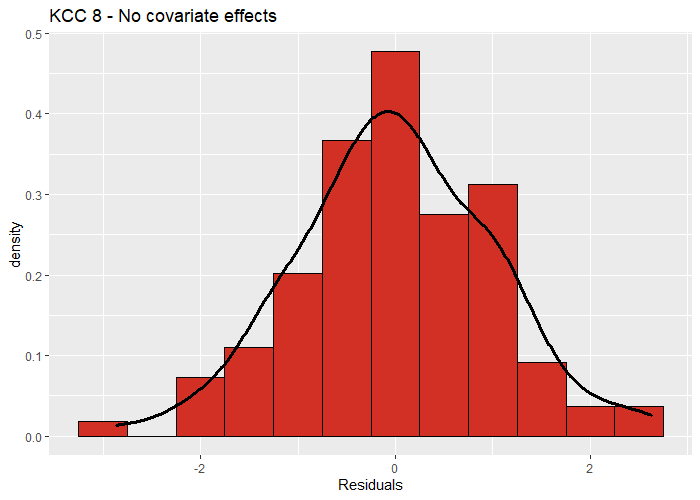
\includegraphics[width=0.45\linewidth]{figures/res_kcc_8_no_covariates.png}
  \caption{Residuals of KCC 8 log-sales fitted to an ex-Gaussian distribution with no covariate effects together with their density curve}
  \label{fig:res_kcc_8_no_covariates}
\end{figure}




Again, Model \ref{eq:gamlss_kcc_2} is applied to the log-sales. The summary output and estimated parameters with confidence intervals can be seen in \autoref{fig:gamlss_kcc_8_estimated_parameters} and in \autoref{tab:nu_ci_kcc_8}. We notice that models fit is acceptable matching the elevated sales during promo weeks and that the variability is strictly decreasing with the overall range having a range between 0.1 and 0.3. Skewness remains low in the data.
\\




%\VerbatimInput[frame = single, label = "GAMLSS Fit on KCC 8" ]{gamlss_fit_kcc_8_try1.txt}

\inputRoutput[caption={GAMLSS Fit on KCC 8}, numbers=left,numberstyle=\tiny, label=output:gamlss_fit_kcc_8_try1]{gamlss_fit_kcc_8_try1.txt}



\begin{figure}[H]
\centering
  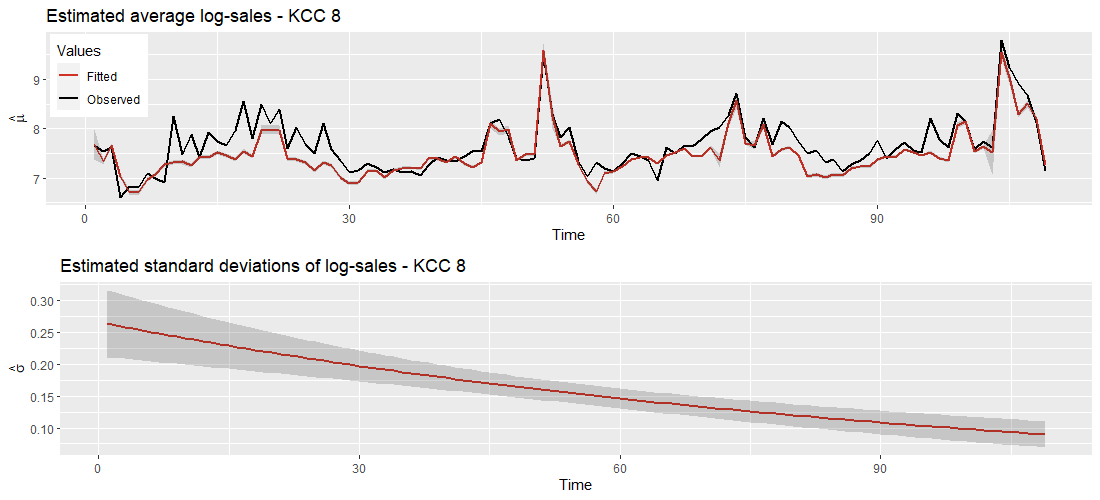
\includegraphics[width=0.95\linewidth]{figures/gamlss_kcc_8_estimated_parameters.png}
  \caption{Estimated location parameter $\hat{\mu}$ compared to the observed values and scale parameter $\hat{\sigma}$ with confidence bands of GAMLSS fit - KCC 8}
  \label{fig:gamlss_kcc_8_estimated_parameters}
\end{figure}



\begin{table}[H]
\setlength\arrayrulewidth{1pt}  
\centering
\begin{adjustbox}{max width=\textwidth}\
\begin{tabular}{|c|c|c|}
\hline
\rowcolor{lightgray} 
Lower & $\hat{\nu}$ & Upper \\ \hline
0.181        & 0.158           & 0.203        \\ \hline
\end{tabular}
\end{adjustbox}
\caption{Estimated skewness parameter $\hat{\nu}$ of GAMLSS fit with 95\% confidence interval bounds - KCC 8}
\label{tab:nu_ci_kcc_8}
\end{table}



Time as well as the total markdown percentage exhibit similar positive effects on the response as in \ac{KCC} 6, collapsing into a straight line. The promo effects seem to be more balanced, with different interquartile ranges for all cases.
\\


\begin{figure}[H]
\centering
  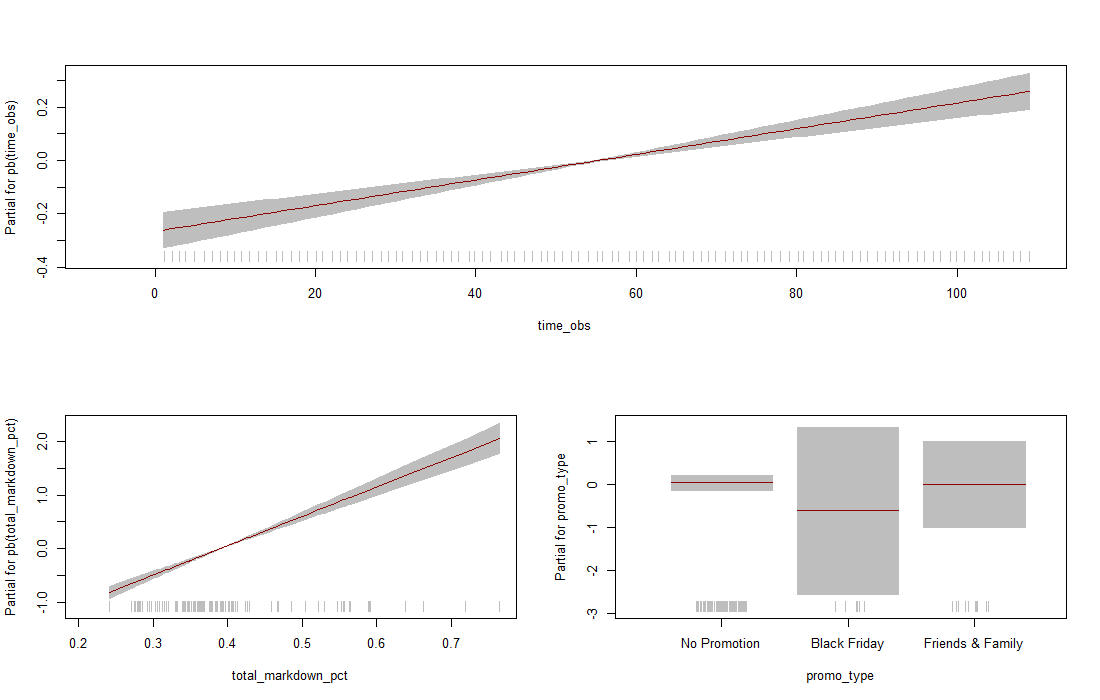
\includegraphics[width=0.95\linewidth]{figures/gamlss_effects_kcc_8.png}
  \caption{Covariate effects on the expected response variable (log-sales) of GAMLSS fit - KCC 8}
  \label{fig:gamlss_effects_kcc_8}
\end{figure}



Looking at \autoref{fig:gamlss_residuals_kcc_8} and the summary output for the distribution of the quantile residuals, the fitting method for this cluster is also justified. The Shapiro-Wilk test is "weaker" in comparison to the fit without covariate effects with a p-value of 0.86, which is still a solid reason to retail the null hypothesis of normality.


\begin{figure}[H]
\centering
  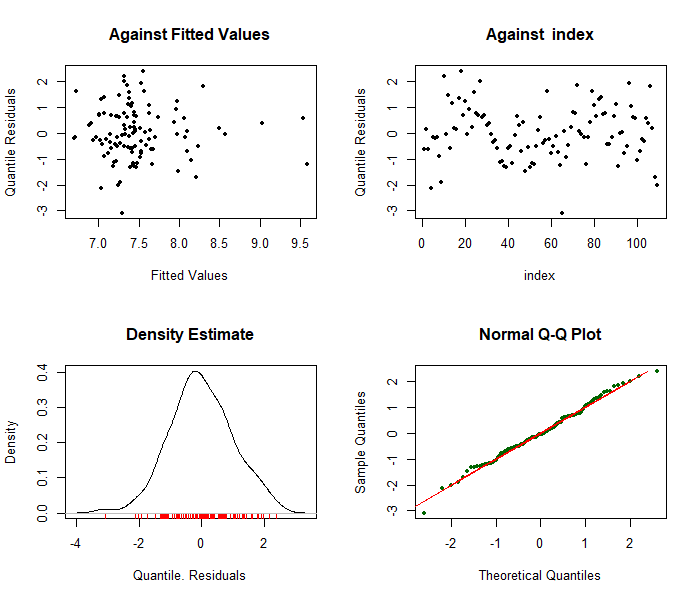
\includegraphics[width=0.95\linewidth]{figures/gamlss_residuals_kcc_8.png}
  \caption{Residuals of GAMLSS fit - KCC 8}
  \label{fig:gamlss_residuals_kcc_8}
\end{figure}


%\VerbatimInput[frame = single, label = "Residuals of GAMLSS Fit on KCC 8" ]{gamlss_residuals_kcc_8.txt}

\inputRoutput[caption={Residuals of GAMLSS Fit on KCC 8},numbers=left,numberstyle=\tiny, label=output:gamlss_residuals_kcc_8]{gamlss_residuals_kcc_8.txt}


